% !TeX root = ../praktikum.tex
% !TeX encoding = UTF-8
% !Tex spellcheck = de_DE

Für die Durchführung des Versuchs wurde ein temperaturgesteuerter cw- Laser mit emittiertem Licht der Wellenlänge 660nm verwendet. Der emittierte Laserstrahl wird in eine Leitungsfaser eingekoppelt.

\begin{figure}[h]
	\centering
	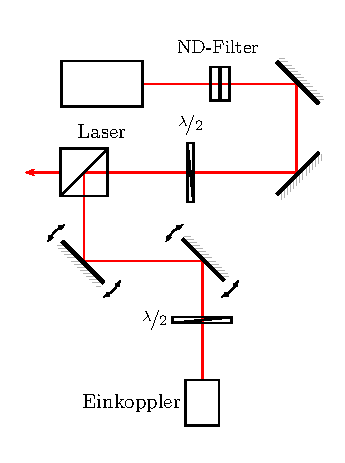
\includegraphics[width=0.5\linewidth]{graphs/versuchsaufbau/lasereinheit}
	\caption[Schematischer Aufbau Lasereinheit]{
		Schematischer Strahlungsaufbau zwischen Laser und Fasereinkopplung. Nach dem Verlassen des Lasers wird die Lichtintensität aus Sicherheitsgründen mit hilfe eines ND-Filters reduziert. Mit Hilfe der draus folgenden Spiegel wurde der Strahlenverlauf feinjustiert. Der Strahlteiler dient dazu, dass je zwei Versuchsaufbauten Licht erhalten. Mit Hilfe der sich davor befindlichen $\nicefrac{\lambda}{2}$- Platte die Intensität des Laserstrahls so eingestellt werden, dass beide Versuchsaufbauten ausreichend Lichtleistung erhalten. Der zweite Strahl nach dem Strahlteiler wird nicht weiter betrachtet.
	}
	\label{fig:lasereinheit}
\end{figure}

Der Faserkopplungsaufbau (siehe Abbildung \ref{fig:lasereinheit}) befindet sich bereits in einem aufgebauten Zustand auf einer eigenen Platte und wurde lediglich optimiert. Der Laser\footnote{Modell  \textit{LD: Mitsubishi ML101J27}. Betrieben wurde der Laser mit 90,3 mA bei $18^\circ C$ und hat einer maximale Leistung von 35 mW.} Zur Regulierung der Intensität wird die Eigenschaft der Polarisation des Lichts ausgenutzt, welche anschaulich als \textit{Schwingungsebene} einer Lichtwelle beschrieben werden kann. Der Laserstrahl durchläuft eine $\nicefrac{\lambda}{2}$- Platte; dabei handelt es sich um eine doppelbrechende Platte, die den beiden entstehenden Teilwellen einen Gangunterschied erteilt, der gleich der Hälfte der Bezugswellenlänge $\lambda$ ist. In Diagonalstellung wird die Polarisation des Lichts gedreht. Letzterer Effekt wird hier genutzt, da so in Kombination mit dem Strahlteiler hinter der  $\nicefrac{\lambda}{2}$- Platte die Intensitätsaufteilung des anschließend verwendeten Lichts reguliert werden kann. Durch Drehung der  $\nicefrac{\lambda}{2}$- Platte vor dem Strahlteiler kann beeinflusst werden, wie hoch der Anteil des Lichts mit der Polarisation ist, welche durch den Strahlteiler zum restlichen Versuchsaufbau gelenkt wird.

Auch vor der Fasereinkopplung spielt die Polarisation eine Rolle, da die lichtleitende Faser für eine bestimmte Polarisation die höchste Effizienz aufweist. \\

Zur Optimierung der Einkopplung des Lichts in die Faser wird ein Laserpointer an dem noch freien Ende der Faser angebracht und vor dem Einkoppler mithilfe der Spiegel eine optimale Überlagerung der beiden Signale eingestellt. So wird das Axiom der Strahlenumkehr der geometrischen Optik genutzt, um den Laser unter dem korrekten Winkel und Ort einzukoppeln. Da jedoch die Laserstrahlen eine räumliche Ausdehnung haben und aufgrund der relativ hohen Lichtintensitätsdichten dir Überlagerung nur schwer zu erkennen ist , wird anschließen die Intensität des aus der Faser austretenden Lichtes beobachtet, um dessen Leistung weiter zu optimieren. Dies erfolgt zunächst mit dem bloßen Auge und anschließend mit einem Powermeter, welches an ein Oszilloskop angeschlossen wird, um schnelle Änderungen der gemessenen Lichtleistung besser sichtbar zu machen. Es wird ein Optimum der Fasereinkopplung möglichst genau eingestellt. 

